\documentclass{article}
\usepackage{graphicx}
\usepackage{subcaption}
\usepackage{float}
\usepackage{listings}
\usepackage{xcolor}
\usepackage{natbib}
\usepackage[utf8]{inputenc}   % Para usar acentuação direta no código
\usepackage[T1]{fontenc}      % Para melhorar a codificação das fontes
\usepackage[portuguese]{babel}    % Ou 'portuguese', mas 'brazil' é preferido

\author{Felipe B. R. Karmann, João M. S. da Silva e Souza}
\date{30 de junho de 2025}
\title{Uso de técnicas de processamento de imagem na identificação de alterações na cobertura vegetal em Blumenau}

\setlength{\oddsidemargin}{-0.5cm} % Margem esquerda
\setlength{\evensidemargin}{-0.5cm} % Margem direita (para documentos de duas páginas)
\setlength{\textwidth}{17cm} % Largura do texto
\setlength{\topmargin}{-1.5cm} % Margem superior
\setlength{\textheight}{24cm} % Altura do texto

\begin{document}

\maketitle

\section{Introdução}
\subsection{Descrição do problema}

A cidade de Blumenau é historicamente vulnerável a enchentes, sendo este fato devido à sua geografia montanhosa, rios urbanos e padrões de chuva intensos. A gestão de riscos naturais requer ferramentas que combinem automação, visão computacional e análise de dados geográficos para monitorar o uso do solo e identificar áreas críticas.

\subsection{Trabalhos-base}

\begin{figure}[H]
  \centering
  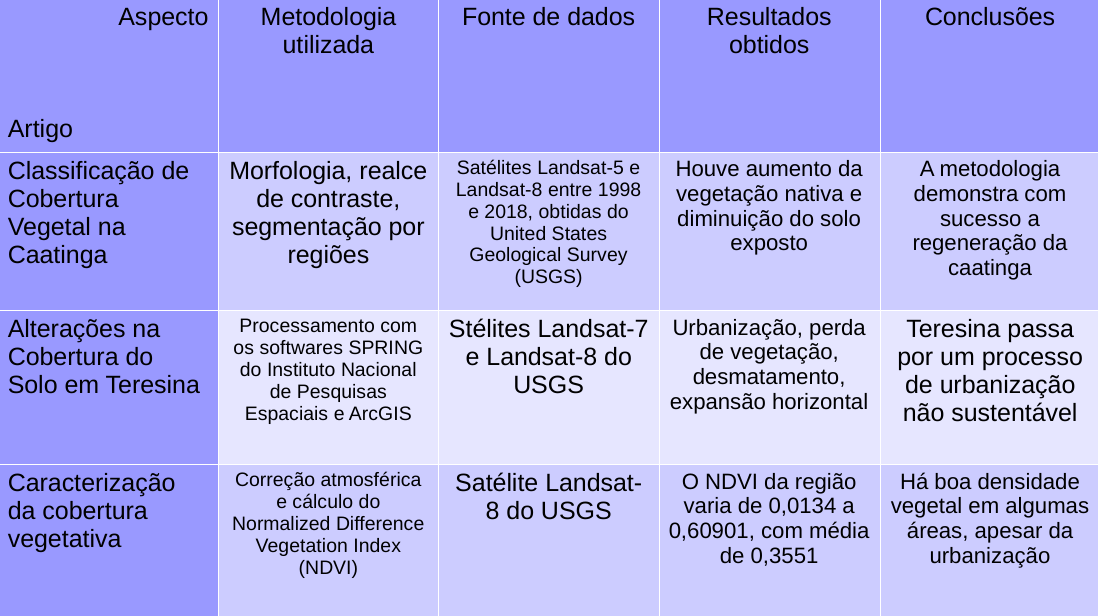
\includegraphics[width=0.8\textwidth]{../tabela.png}
  \caption{Tabela comparativa dos trabalhos-base deste estudo.}
  \label{Tabela comparativa}
\end{figure}

A partir dos artigos escolhidos para servir de base para o nosso trabalho, o problema a ser resolvido é a criação de um algoritmo que detecte padrões e características do terreno em fotos tiradas por satélites, e, usando técnicas de processamento de imagem, identifique alterações na cobertura vegetal de áreas que sofreram desastres naturais.

A lógica da separação da vegetação em diferentes níveis de densidade baseada em imagens de momentos diferentes foi inspirada nas técnicas descritas por Nóbrega \textit{et al}. (2023)\cite{artigo01}, que reforçam a eficácia da classificação espectral na identificação de alterações no solo.

A estratégia de comparar imagens de diferentes anos com o objetivo de avaliar a perda de cobertura vegetal foi fundamentada nas práticas descritas por Lima \textit{et al}. (2021)\cite{artigo03}, cujo trabalho evidenciou os impactos da urbanização por meio de processamento digital de imagens.

O uso de indicadores visuais para medir a cobertura vegetal, como o NDVI abordado por Barros {et al}. (2020)\cite{artigo02}, foi importante para embasar a importância da detecção automática de alterações no solo em áreas urbanas vulneráveis.

As técnicas de segmentação, binarização, análise multitemporal e classificação supervisionada usadas nos artigos serviram de inspiração direta para o pipeline da nossa solução, especialmente a separação por tonalidade, a subtração temporal e o uso de máscaras para destacar mudanças.

\section{Fonte dos dados}

A base de imagens foi criada por nós a partir de fotos de satélite da região de Blumenau obtidas no serviço Google Earth, com foco em áreas com grande cobertura vegetal. Para obter fotos do mesmo lugar em datas diferentes, usamos a funcionalidade ``imagens históricas''; para cada área selecionada, tiramos duas fotos, uma do dia 19 de abril de 2023 e outra do dia 17 de abril de 2025, tendo, portanto, quase exatamente dois anos de diferença. As fotos foram tiradas de uma altitude considerada por nós apropriada para a detecção de diferenças na cobertura vegetal e têm, todas elas, tamanho 512x512.

A equipe tomou o devido cuidado para garantir que cada par de fotos tivesse a mesma posição no mapa para que não houvesse diferenças que não aquelas causadas pela passagem do tempo.

\section{A pipeline}

O nosso algoritmo pode ser dividido em cinco etapas básicas, cada uma consistindo numa técnica de processamento de imagens vista em sala de aula:
\begin{itemize}
  \item Segmentação (\texttt{MeanShift.py}): usamos o algoritmo Mean Shift para segmentar a imagem obtida em regiões de cores diferentes, tendo por base o valor médio da intensidade de cada região. Os resultados desta etapa se mostraram precisos para a detecção de cobertura vegetal em áreas urbanas, uma vez que estas têm seu próprio esquema de cores facilmente distinguível de todo o resto (prédios, ruas, água, solo exposto, etc.) O script pergunta ao usuário pelo parâmetro quantil desejado; para os exemplos deste trabalho, usamos sempre 0,1. Esta etapa não é indispensável; a binarização sozinha é suficiente para destacar a vegetação em muitos casos, mas a segmentação ajuda a eliminar ruídos e sombras, garantindo assim um resultado mais preciso;
  \item Binarização (\texttt{Binarizar.py}): esta etapa se mostrou necessária por conta de diferenças que inevitavelmente existem entre duas fotos tiradas por satélite em momentos diferentes, normalmente relacionadas à hora do dia em que são tiradas, à qualidade da câmera usada ou à presença de filtros. Para normalizar o padrão de cores entre imagens, o algoritmo escolhe automaticamente o limiar usado na binarização calculando o nível médio de intensidade da imagem. Observamos que, invariavelmente, as áreas vegetais tornavam-se a parte escura da imagem, e todo o resto a parte clara;
  \item Subtração (\texttt{Subtrair.py}): em seguida, fazemos a subtração das duas imagens, cada uma representando o mesmo lugar em momentos diferentes;
  \item Erosão e dilatação (\texttt{Abertura.py}): agora, já obtivemos a diferença exata entre as duas imagens, representadas, no resultado da subtração, pelas regiões brancas. No entanto, devido à diferença que tende a existir entre duas imagens quaisquer, é provável que a maioria das regiões brancas represente não mais do que um pequeno acidente de fotografia, como uma sombra. Por isto, decidimos aplicar uma combinação de erosão e dilatação usando um elemento estruturante de tamanho 3 (também estudamos outros tamanhos, e o valor é escolhido no momento da execução do script). Desta maneira, regiões brancas insignificantes são eliminadas na erosão e não têm chance de retornar na dilatação, deixando apenas regiões significativas que possuem alto valor semântico para a análise de efeitos dos desastres naturais;
  \item Aplicação de máscaras (\texttt{AplicarMascara.py}): esta etapa pode ser vista como opcional; seu único propósito é facilitar a leitura do resultado. A partir do resultado da etapa anterior, as regiões brancas são transformadas em máscaras, que são em seguida aplicadas à imagem original para assinalar as regiões de interesse.
\end{itemize}

\section{Trechos de código}

Conforme mencionado anteriormente, nossa solução é dividida em cinco etapas básicas, que foram escritas cada uma em seu próprio arquivo; desta maneira, pudemos testar cada etapa do algoritmo separadamente. A entrada usada em cada arquivo é a saída gerada pela etapa anterior.

Começando pela parte que, do ponto de vista da codificação, foi a mais delicada, a Mean Shift (alguns trechos de código e linhas em branco foram removidos desta amostra para poupar espaço no documento):

\subsection{Mean Shift}

\begin{verbatim}
        imagem = Image.open(caminho_imagem).convert('RGB')
        array_img = np.array(imagem)
        array_img = redimensionar_imagem(array_img)
        img_flat = array_img.reshape(-1, 3)

        largura_banda = estimate_bandwidth(img_flat, quantile=quantil, n_samples=amostras)
        largura_banda = max(largura_banda, 0.1)
        ms = MeanShift(bandwidth=largura_banda, bin_seeding=True)
        ms.fit(img_flat)

        rotulos = ms.labels_
        centros = ms.cluster_centers_
        num_clusters = len(np.unique(rotulos))
        print(f"Número de clusters encontrados: {num_clusters}")

        img_segmentada = centros[rotulos].reshape(array_img.shape)
        img_segmentada = np.clip(img_segmentada, 0, 255).astype(np.uint8)
        Image.fromarray(img_segmentada).save(caminho_saida)

        return num_clusters
\end{verbatim}

O código transforma a imagem em uma matriz plana de pixels RGB, estima a largura de banda para o algoritmo Mean Shift e executa a segmentação agrupando pixels com base na similaridade de cor. Cada pixel da imagem é então substituído pelo centroide do seu respectivo cluster, resultando em uma imagem segmentada com regiões homogêneas de cor.

\subsection{Binarização}

\begin{verbatim}
    imagem = carregar_imagem_em_cinza(caminho_imagem)
    limiar = calcular_limiar_automatico(imagem)
    binarizada = binarizar_imagem(imagem, limiar)
    cv2.imwrite(caminho_saida, binarizada)
\end{verbatim}

O algoritmo de binarização carrega a imagem em escala de cinza, calcula o limiar automaticamente como a média dos valores de intensidade dos pixels e aplica a binarização usando este limiar: pixels acima viram branco (255), abaixo viram preto (0).

\subsection{Subtração}

\begin{verbatim}
    imagem_depois = redimensionar_para_compatibilidade(imagem_antes, imagem_depois)
    diferenca = cv2.absdiff(imagem_antes, imagem_depois)

    return diferenca
\end{verbatim}

O algoritmo calcula a diferença absoluta entre duas imagens, pixel a pixel, resultando em uma nova imagem que destaca as alterações entre elas.

\subsection{Abertura}

\begin{verbatim}
    kernel = np.ones((kernel_size, kernel_size), np.uint8)
    return cv2.morphologyEx(imagem, cv2.MORPH_OPEN, kernel)
\end{verbatim}

O algoritmo de erosão e dilatação utiliza um elemento estruturante (ou kernel) do tamanho escolhido pelo usuário e aplica a operação de abertura morfológica, erosão seguida de dilatação. Esta operação remove pequenos regiões brancas enquanto mantém as principais, conforme explicado na seção anterior.

\subsection{Aplicação de máscaras}

\begin{verbatim}
    resultado = imagem.copy()

    for mascara in mascaras:
        regiao = cv2.bitwise_and(imagem, imagem, mask=mascara)
        hsv = cv2.cvtColor(regiao, cv2.COLOR_BGR2HSV)
        hsv[:, :, 1] = 255
        hsv[:, :, 2] = np.where(mascara > 0, 255, hsv[:, :, 2])

        regiao_realcada = cv2.cvtColor(hsv, cv2.COLOR_HSV2BGR)
        resultado = cv2.addWeighted(resultado, 1, regiao_realcada, 0.7, 0)

    return resultado
\end{verbatim}

O algoritmo aplica máscaras sobre a imagem original, realçando visualmente as regiões mascaradas com aumento da saturação e brilho. As demais regiões da imagem permanecem inalteradas.

\section{Exemplo de resultados}

Para esta demonstração, usaremos duas imagens da região central de Blumenau, uma de 2023 e outra de 2025:

\begin{figure}[H]
    \centering
    \begin{subfigure}[b]{0.48\textwidth}
        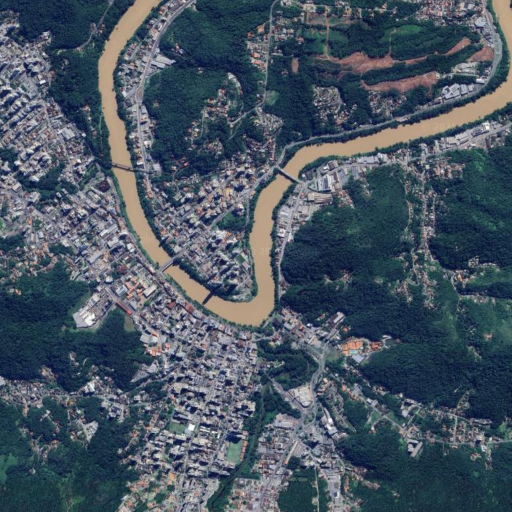
\includegraphics[width=\textwidth]{../Imagens/012023.png}
        \caption{O centro de Blumenau em 2023.}
        \label{2023}
    \end{subfigure}
    \hfill % Espaço entre as imagens
    \begin{subfigure}[b]{0.48\textwidth}
        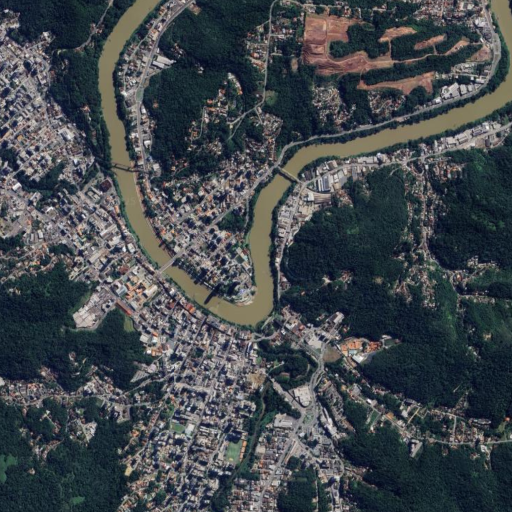
\includegraphics[width=\textwidth]{../Imagens/012025.png}
        \caption{O centro de Blumenau em 2025.}
        \label{2025}
    \end{subfigure}
    \caption{As fotos originais.}
    \label{original}
\end{figure}

Como é fácil notar, as imagens possuem diferença significativa no nível de intensidade. Nós atribuímos a causa provável disto à hora do dia e às condições de iluminação natural.

Conforme explicado anteriormente, o próximo passo é a clusterização das imagens usando o algoritmo Mean Shift com parâmetro quantil de 0,1:

\begin{figure}[H]
    \centering
    \begin{subfigure}[b]{0.48\textwidth}
        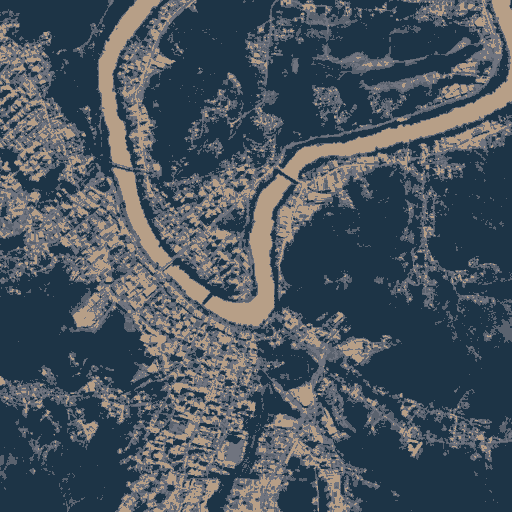
\includegraphics[width=\textwidth]{../Imagens/012023_mean_shift.png}
        \caption{A foto de 2023 segmentada.}
        \label{2023}
    \end{subfigure}
    \hfill % Espaço entre as imagens
    \begin{subfigure}[b]{0.48\textwidth}
        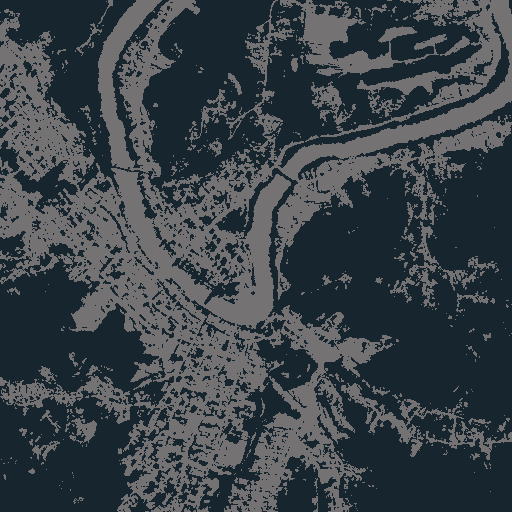
\includegraphics[width=\textwidth]{../Imagens/012025_mean_shift.png}
        \caption{A foto de 2025 segmentada.}
        \label{2025}
    \end{subfigure}
    \caption{Resultado da aplicação do Mean Shift.}
    \label{segmentada}
\end{figure}

Vale notar que a segmentação da imagem de 2023 assinalou muitas pequenas regiões da cidade com a mesma cor que a água do rio. Isto não será um problema; o algoritmo de binarização destacará a porção vegetal de todas as regiões mais claras:

\begin{figure}[H]
    \centering
    \begin{subfigure}[b]{0.48\textwidth}
        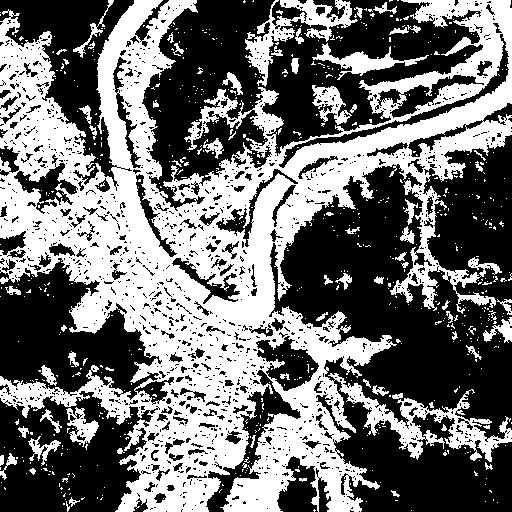
\includegraphics[width=\textwidth]{../Imagens/012023_bin.png}
        \caption{A foto de 2023 binarizada.}
        \label{2023}
    \end{subfigure}
    \hfill % Espaço entre as imagens
    \begin{subfigure}[b]{0.48\textwidth}
        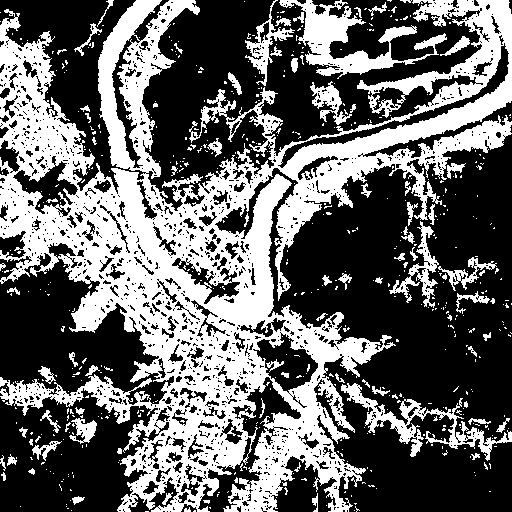
\includegraphics[width=\textwidth]{../Imagens/012025_bin.png}
        \caption{A foto de 2025 binarizada.}
        \label{2025}
    \end{subfigure}
    \caption{Resultado da binarização.}
    \label{binarizada}
\end{figure}

Finalmente, é o momento de fazer a subtração das duas imagens para apontar diferenças na cobertura vegetal entre estes dois anos. Como explicado anteriormente, há a presença de muitas pequenas regiões claras no resultado, o que por sua vez resulta em parte da diferença de intensidade entre as duas imagens e noutra parte de fatores não naturais (corte intencional de árvores, por exemplo). Por este motivo, aplicamos o algoritmo de erosão e dilatação com kernel de tamanho 3 para eliminar diferenças consideradas insignificantes. Abaixo o resultado:

\begin{figure}[H]
    \centering
    \begin{subfigure}[b]{0.48\textwidth}
        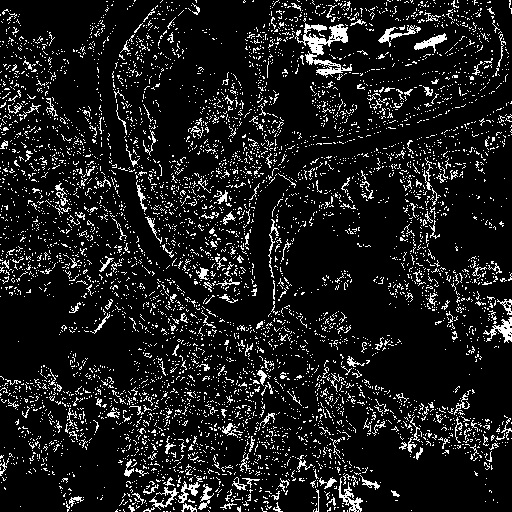
\includegraphics[width=\textwidth]{../Imagens/012025_sub.png}
        \caption{O resultado da subtração das imagens.}
        \label{2023}
    \end{subfigure}
    \hfill % Espaço entre as imagens
    \begin{subfigure}[b]{0.48\textwidth}
        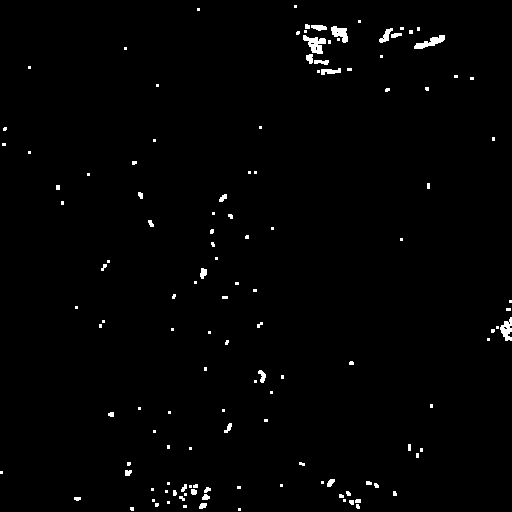
\includegraphics[width=\textwidth]{../Imagens/resultado01.png}
        \caption{A imagem ao lado após a erosão e a dilatação.}
        \label{2025}
    \end{subfigure}
    \caption{Isolando regiões de interesse.}
    \label{resultado}
\end{figure}

A partir da última figura, podemos observar que a maior região de interesse está na região norte da imagem. Conferindo nas imagens originais, é possível verificar que houve, entre 2023 e 2025, um aumento significativo na porção de solo exposto naquela região, em prejuízo da cobertura vegetal.

Por motivos de limite no número de páginas do relatório, não mostraremos os resultados da etapa de aplicação de máscaras, mas as imagens serão entregues com o trabalho e podem ser consultadas. Observando-as, verficica-se que o contraste com o fundo marrom do solo exposto, somado ao efeito de transparência da máscara, lhe confere um tom vermelho, o que também serve para indicar a principal região de interesse. Ao mesmo tempo, as diferenças presentes na malha urbana são assinaladas em azul, e em verde (turquesa) as diferenças de tipos vegetais (florestas em oposição a pastos, por exemplo). Isto, é claro, é um acidente surgido do contraste entre o solo e a máscara, mas pode ser aproveitado para facilitar a interpretação dos resultados.

\section{Conclusão}

O nosso algoritmo mostrou-se eficaz na identificação de alterações na cobertura vegetal; a sua combinação estratégica de técnicas simples do processamento de imagem tem o potencial de ajudar profissionais a analisar os efeitos de desastres naturais.

\bibliographystyle{plain}
\bibliography{referencias}

\end{document}
